\documentclass{standalone}\usepackage{tikz}\usetikzlibrary{automata, positioning, arrows, shapes, fit, arrows.meta}\begin{document}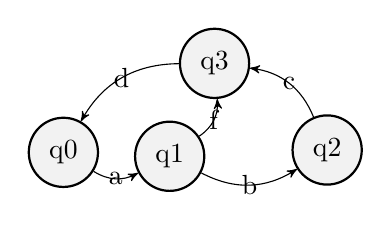
\begin{tikzpicture}\tikzset{->,>=stealth',node distance=6cm,every state/.style={thick, fill=gray!10}, initial state/.style={thick, fill=gray!10, fill=yellow}initial text=$ $, }
	\node[state] (0) at (0.84,0.68) {q0};
	\node[state] (1) at (2.19,0.63) {q1};
	\node[state] (2) at (4.19,0.71) {q2};
	\node[state] (3) at (2.7600000000000002,1.81) {q3};
	\path (3) edge[bend right] node {d} (0);
	\path (0) edge[bend right] node {a} (1);
	\path (1) edge[bend right] node {f} (3);
	\path (1) edge[bend right] node {b} (2);
	\path (2) edge[bend right] node {c} (3);\end{tikzpicture}\end{document}